\section{Theory \& Methods}
\subsection{Theory}
\subsubsection{Automation Pyramid}
The automation pyramid is a graphical representation of the different levels of
automation in a factory or industry, as seen in Figure \ref{figure:ap}.

\begin{figure}[ht]
	\centering 
	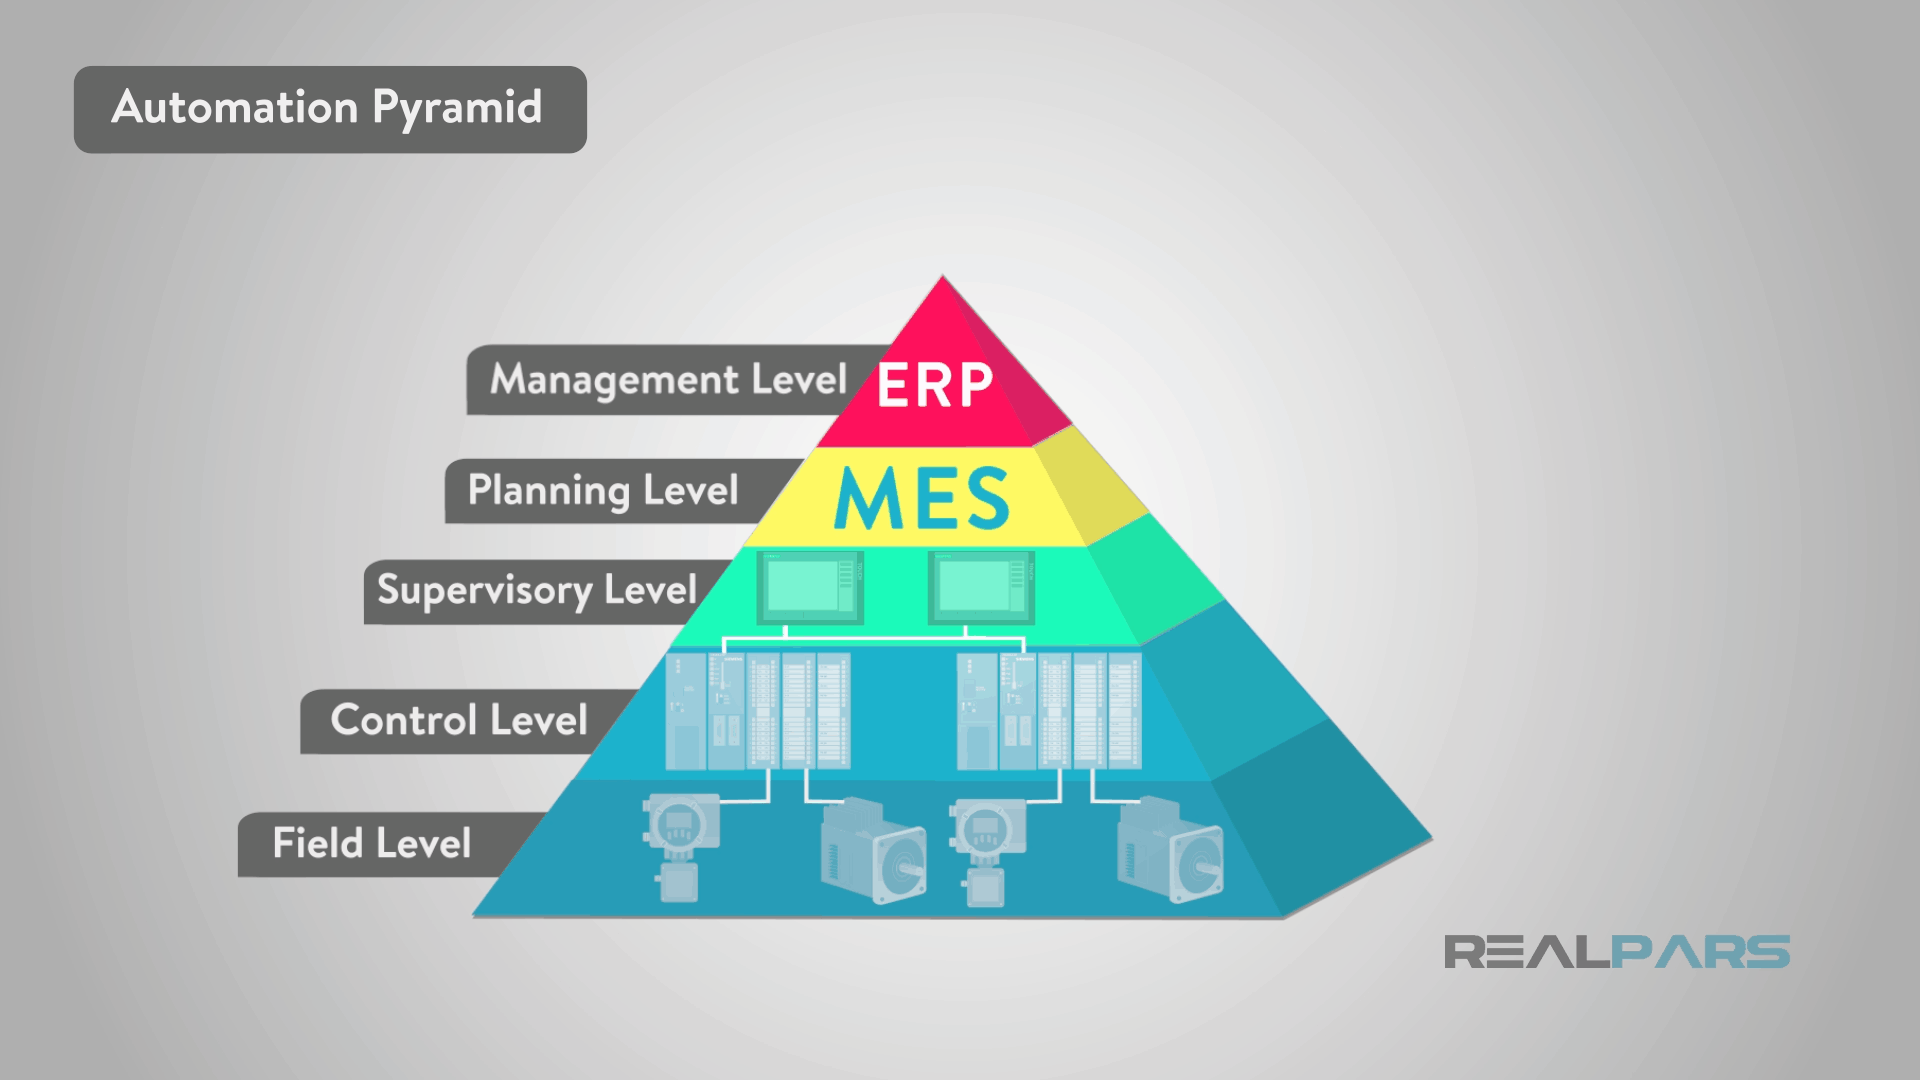
\includegraphics[width=1\linewidth]{images/automation_pyramid}
	\caption{Illustration of the Automation Pyramid}
	\label{figure:ap}
\end{figure}


The first level, the field level, consists of the devices, actuators, and
sensors that are used on the production floor. The control level is where PLCs
(Programmable Logic Controller) and PIDs (Proportional-Integral-Derivative
controller) are located. These are used to control the devices in the field
level. The third layer, the supervisory level, utilises SCADA. SCADA
is an abbreviation of Supervisory Control And Data Acquisition. This level
combines the previous level and makes it possible to control the system from
a single location. Above the supervisory level is the planning level. It is on
this level the computer management system MES, Manufacturing Execution System,
is located. The MES makes it possible to monitor the manufacturing process in
the factory from start to finish. The top layer of the pyramid is the management
level. On this level, the ERP, Enterprise Resource Planning, a management system
is located, making the company's management able to control their operations. \cite{ap}\\

This project evolves around the fourth layer of the pyramid, the planning level,
as the given task is to develop an MES for Refslevbæk Bryghus A/S, to control
and optimise their brewery. 


\subsubsection{Overall Equipment Effectiveness}
The \textbf{O}verall \textbf{E}quipment \textbf{E}ffectiveness, OEE, is a
measurement of how effective a given production line is. It identifies what
percentage of the manufacturing time that is fully utilised. The formula for
the OEE can be seen in Equation \ref{eq:OEE}
\begin{equation} \label{eq:OEE}
    OEE = \frac{Good Count \cdot Ideal Cycle Time}{Planned Produciton Time}
\end{equation}

Where \textit{Good Count} is the amount of acceptable products produced,
\textit{Ideal Cycle Time} is the theoretical minimum time to produce a single
product and \textit{Planned Production Time} is the total time that the
manufacturing process is scheduled for production. \cite{oee}

\subsubsection{Optimal Production Speed}
When finding the optimal production speed, several test batches need to have
been produced. This is to have data points to plot. The values for the
\(x\)-axis is the normalised machine speed and the values for the \(y\)-axis is
the calculated OEE. When all data points have been plotted, a third-degree
polynomial trend line, line of best fit, is applied. Polynomial trending
describes a pattern in data that is curved to fit the points.\\

To find the slope of the function, in this case, the trend line, the derivative
is calculated. To find the extrema (minima and maxima) of the function, the
expression is solved for \(x\) where \(y = 0\). This gives all the \(x\)-values
for which the slope is zero. To check if it is a local minimum or local maximum
that has been found (for the \(x\)-value), the second derivative needs to be
calculated.\\

The second derivative is then solved for \(y\) where \(x = found Value\). If the
result is greater than zero, the extremum at the given \(x\)-value is a local
minimum and if the result is less than zero, the extremum at the given 
\(x\)-value is a local maximum.\\ \cite{ops}

When optimising, the goal is to find the \(x\)-value with the greatest
\(y\)-value, which is why the local maximum for the trend line is the optimal
production speed for the machine. 


\subsection{Methods}
\subsubsection{Unified Process}
Unified Process, UP, is a an iterative and incremental software development
process framework. UP consist of four phases \cite{up}: 

\myparagraph{The Inception Phase}
The inception phase is the first phase in UP, and it is in this phase that it
is determined whether the system can be developed or not. In this phase it is
decided which responsibilities the system has and where important requirements
and critical risks are identified. 

\myparagraph{The Elaboration Phase}
In the elaboration phase, iterative development is used to make the requirements,
design, analysis, and test from the requirements specification and the priority
that has been made. In this phase Scrum will be used to manage the iterations.

\myparagraph{The Construction Phase}
In the construction phase, the development of the system takes place. Here, 
unified modelling language will be used to identify which classes and components
the system will consist of. 

\myparagraph{The Transition Phase}
In the transition phase, it will be verified that all the agreed upon
functions are implemented and the customer will answer if they are satisfied
with the developed system.


\subsubsection{Scrum}
To keep track of the group work, the Scrum framework, with a few exceptions, is
used. Scrum consists of multiple artefacts and ceremonies, and in this project
product roadmap, Scrum meetings, product and sprint backlogs and burndown charts
will be used.\cite{scrum} Each sprint will have a duration of two weeks and the issues for
the sprint backlog will be chosen at the beginning of each sprint, at the Scrum
meeting. The Scrum meeting will take place each Friday and will be a mixture of
sprint planning, daily Scrum, and sprint review. To manage Scrum, ZenHub, a
management solution that can be integrated with GitHub, is used. On ZenHub the
group will create the roadmap, that acts as a schedule for the project and
board, which is where the issues will be handled. A burndown chart for each
sprint is automatically generated and kept up to date by ZenHub. The board will
consist of five columns, as seen below.

\begin{table}[H]
    \captionof{table}{Scrum Board}
    \begin{tabularx}{\textwidth}{|>{\RaggedRight}X|>{\RaggedRight}X|>{\RaggedRight}X|>{\RaggedRight}X|>{\RaggedRight}X|>{\RaggedRight}X|>{\RaggedRight}X|}
        \hline                             
        \textbf{Product Backlog} & \textbf{Sprint Backlog} & \textbf{In Progress} & \textbf{Review/QA} & \textbf{Closed} \\
        \hline
        Issues & Issues for the given sprint & Issues that is currently being worked on & Issues that are pending (or in) review & Approved issues that have been merged    \\
        \hline
    \end{tabularx}
    \label{table:scrum}
\end{table} 

\subsubsection{MoSCoW}
MoSCoW is an important prioritising model used in software development, as it
describes which parts of the system that constitute the minimal viable product,
MVP. The use cases for the system to be developed are prioritised with the
costumer as this makes it clear which parts of the system to develop first. \cite{moscow}
These use cases are then presented in a table, to improve readability.\\

MoSCoW is an acronym standing for:\\

\begin{description}
    \item [Must have:] the use cases needed for the system to work and be
    accepted by the customer.

    \item [Should have:] what use cases the customer would like to have
    implemented, but they are not necessarily important for the system to work.

    \item [Could have:] use cases the customer would like to have implemented if
    there is enough time for it.

    \item [Won't have (this time):] use cases that is not to be prioritised in
    this iteration, but maybe in future releases.
\end{description}

\subsubsection{FURPS+}
FURPS+ is a model for classifying functional and non-functional requirements and
help giving a detailed description of the requirements. \cite{furps} The acronym stands for: 

\begin{description}
    \item [Functionality:] What the customer wants, including security measures.

    \item [Usability:] How effective is the product from the user's point of
    view? Is the product aesthetically acceptable? Is the documentation adequate?

    \item [Reliability:] What is the most acceptable system downtime? Are system
    errors predictable? Is it possible to demonstrate how accurate the results
    are? How is the system restored?

    \item [Performance:] How fast should the system be? What is the maximum
    response time? What is the throughput? How much memory does the system use?

    \item [Supportability:] Can the system be tested? Is it possible to
    configure the system, expand it, install it, and provide service on the
    system.
\end{description}

The + sign stands for supplementary needs the customer could have, and includes:

\begin{description}
    \item [Design constraints:] Do I/O devices or database management systems
    influence how the software should be built?

    \item [Implementation requirements:] Are there any standards the programmers
    must adhere to? is test-driven development necessary?

    \item [Interface requirements:] What downstream feeds need to be made? What
    other systems should the system work with?

    \item [Physical requirements:] What hardware should the system be
    implemented on?
\end{description}
